\section{Introduction}

In this project it would be analyzed the structure of a typical aircraft wing
composed of front and rear spars and ribs as is shown in the following figure
\ref{fig:wing_structure}.

\begin{figure}[h]
	\centering
	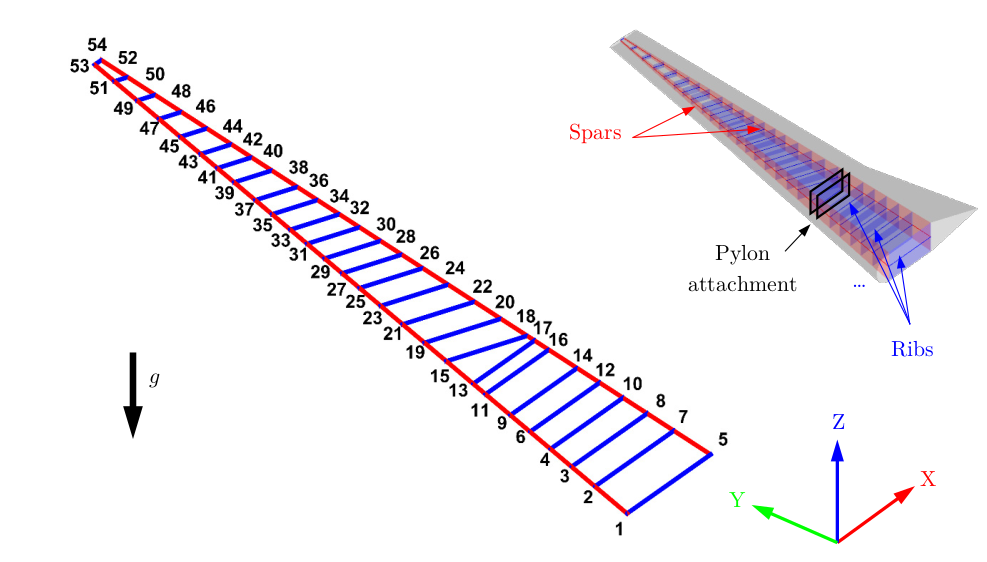
\includegraphics[width=\textwidth]{img/structural_wing.png}
	\caption{Structural representation of the wing}
	\label{fig:wing_structure}
\end{figure}

All the bars (spars and ribs) are considered to have the same shape, showed in figure
\ref{fig:cross_section}. The rotation angles are also showed in figure \ref{fig:angles}.

\begin{figure}[h]
	\centering
	\begin{subfigure}{0.45\textwidth}
		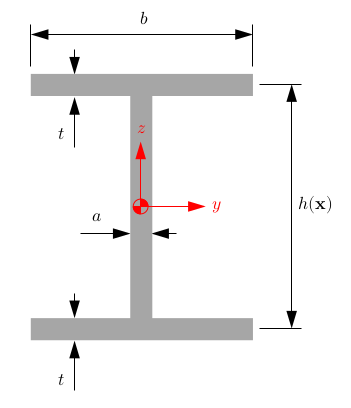
\includegraphics[width=\textwidth]{img/cross_section}
		\caption{Cross section of the bars}
		\label{fig:cross_section}
	\end{subfigure}
	~ %add desired spacing between images, e. g. ~, \quad, \qquad, \hfill etc.
	%(or a blank line to force the subfigure onto a new line)
	\begin{subfigure}{0.45\textwidth}
		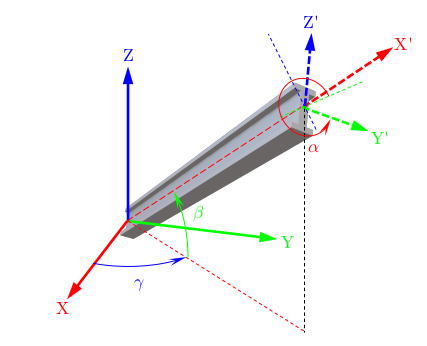
\includegraphics[width=\textwidth]{img/angles.png}
		\caption{Representation of the rotation angles}
		\label{fig:angles}
	\end{subfigure}
	\caption{Definition of bars shape and angles}
	\label{fig:bars_and_angles}
\end{figure}

\section{Code structure}

All the input data is given by the Matlab script \textbf{input\_wing.m}, nodal
coordinates, nodal connectivities, material connectivities and geometrical
parameters.

On this structure some forces will be applied in order to compute the displacements,
and stresses.

\begin{itemize}
	\item Firstly the wing will be attached to the fuselage at nodes 1 and 5,
	which will be fixed.

	\item The weight of the wing will be estimated using the total mass of the wing.
	The effective density of the wing will be:
	\begin{equation}
		\rho^{eff}=\rho^e + \hat{\rho}
	\end{equation}
	, where $\rho^e$ corresponds to the material density of the rib/spar,
	and $\hat{\rho}$ is a pseudo-density accounting for the mass of the rest
	of the wing elements, that can be estimated as
	\begin{equation}
		\hat{\rho} = \frac{M_w - M_s - M_r}{V_s + V_r}
	\end{equation}
	with $M_w =$ 1000 kg being the mass of the whole wing, $M_s$ and $M_r$ the
	mass of the spars and ribs, respectively, while $V_s$ and $V_r$ refer to
	their corresponding total volume.

	\item The aerodynamic forces are considered as in the next figure
	\ref{fig:drag_lift}, where are also shown the expression for obtaining the
	values of drag and lift in every point of the wing:
	\begin{figure}[h]
		\centering
		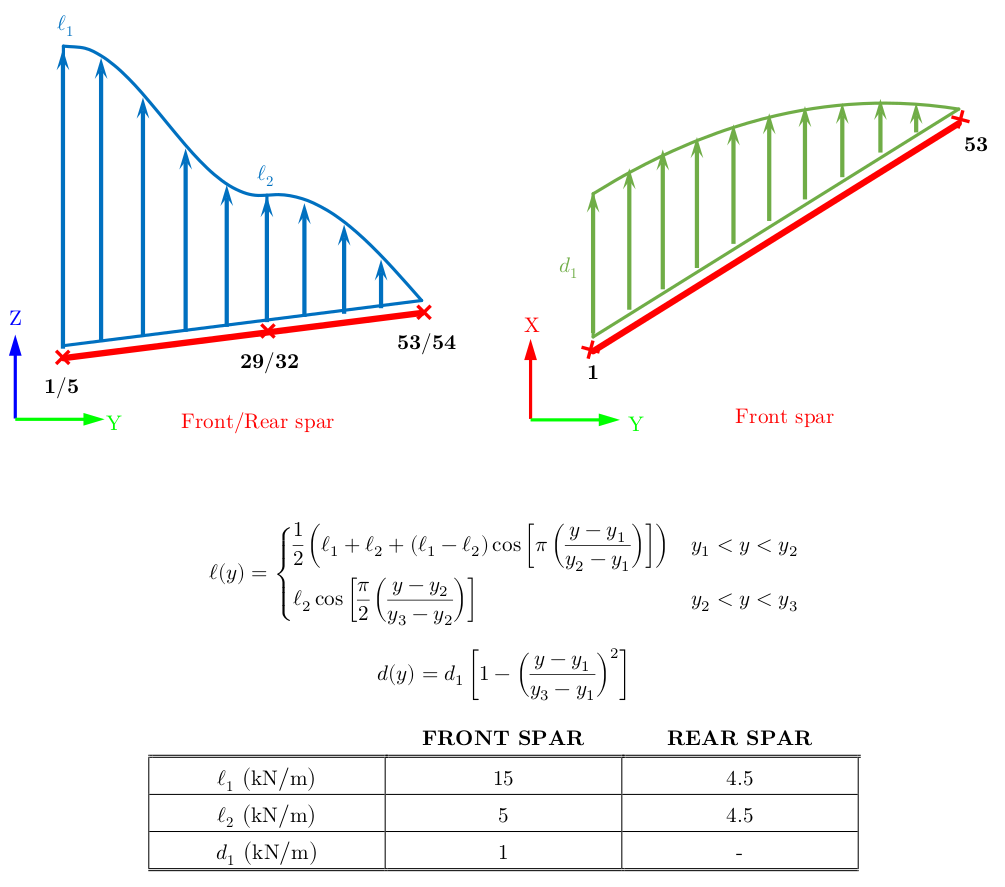
\includegraphics[width=\textwidth]{img/drag_lift.png}
		\caption{Aerodynamic forces applied to the structure}
		\label{fig:drag_lift}
	\end{figure}

	\item The thrust $T_e$ and weight $W_e$ of the engine is transmitted
	through the pylon as a distributed load into ribs \textbf{11}-\textbf{16}
	(element \textbf{7}) and \textbf{13}-\textbf{17} (element \textbf{8}), as
	shown in the figure \ref{fig:engine}:
	\begin{figure}[h]
		\centering
		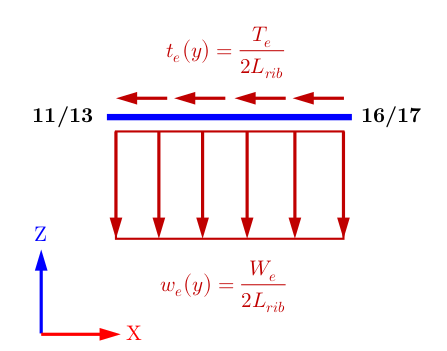
\includegraphics[width=0.45\textwidth]{img/engine.png}
		\caption{Weight and trust of the engine}
		\label{fig:engine}
	\end{figure}
	The value of $T_e$ should be such to compensate the total drag of the wing.
	The mass of the engine is $M_e = 1000 kg$.

\end{itemize}

Considering this forces and constraints, the code will have the following structure:
\begin{enumerate}
	\item For each element it will be calculated its (a) length, (b) section area,
	(c) inertia, (d) torsion constant, (e) volume and (f) mass.

	\item Compute $V_r$, $V_s$, $M_r$ and $M_s$, and compute the pseudo-density
	$\hat{\rho}$, and then the effective density $\rho^{eff}$.

	\item Calculate the thrust of the engine that compensate the total drag.

	\item Compute the stiffness matrix for each element and assembly this into
	the global one.

	\item Compute the force vector for each element and assembly the global
	force vector.

	\item Solve the system $[\mathbf{K}][\mathbf{u}] = [\mathbf{f}]$, considering
	the fixed degrees of freedom, and obtain the displacements and rotations vector.

	\item Obtain the local displacements, rotations and internal forces of each
	element: (a) axial displacements, (b) deflections, (c) rotation angles,
	(d) axial force, (e) shear forces, (f) bending moments and (g) torsion moment.

	\item Plot the results using \textbf{plotWing.m} function.
\end{enumerate}

\newpage

\section{Results}

After running the code, the following results can be obtained (Table \ref{tab:nominal}):

\begin{table}[h]
\centering
\begin{tabular}{ccc}
\hline
\textbf{Parameter} & \textbf{Value} & \textbf{Units} \\ \hline
Total mass	&  19620 	& Kg	\\ \hline
Total lift	&  113725 	& N	\\ \hline
Total drag	&  9.905 	& kN	\\ \hline
Total thrust	&  9.905 	& kN	\\ \hline
\end{tabular}
\caption{Global results}
\label{tab:nominal}
\end{table}

Also the reactions at nodes 1 and 5 where the wing is attached to the fuselage
has been computed:

\begin{table}[h]
\centering
\begin{tabular}{cccc}
\hline
\textbf{Degree of freedom} & \textbf{Node 1} & \textbf{Node 2} & \textbf{Units} \\ \hline
X	  	& -3748,321	& 4478,070	& N 	\\ \hline
Y	  	& -9631,034	& 9631,034	& N 	\\ \hline
Z	  	& 26375,077	& 8773,069	& N 	\\ \hline
$\alpha$   	& -15940,325	& -72662,667	& N/m 	\\ \hline
$\beta$	   	& 8701,091	& 26514,243	& N/m 	\\ \hline
$\gamma$   	& -1478,566	& -1496,513	& N/m 	\\ \hline
\end{tabular}
\caption{Reactions at wing joints}
\label{tab:reactions}
\end{table}

The code also is able to plot some results. In figure \ref{fig:displacements}
are shown the displacements of every node. It can be observed that the maximum
displacement is produced at the tip of the wing with a value of 0.4445 m, and is
mainly in the positive z-component.

\begin{figure}[h]
	\centering
	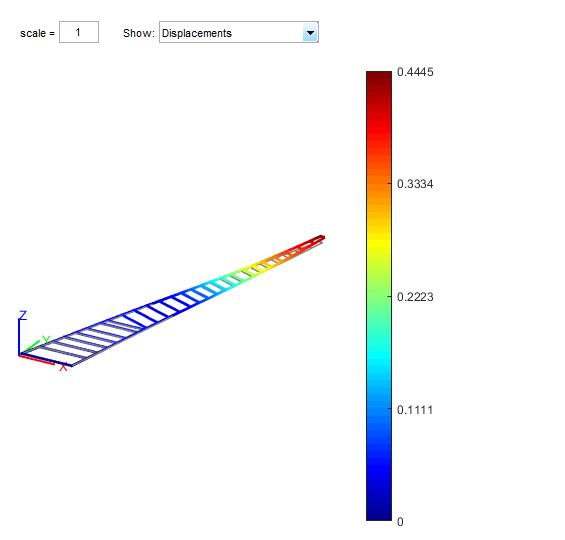
\includegraphics[width=0.6\textwidth]{img/Displacements.jpg}
	\caption{Wing displacements (m)}
	\label{fig:displacements}
\end{figure}

The rest of figures from \ref{fig:axial_disp} to \ref{fig:bending} show other
results given by the code.

\begin{figure}[h]
	\centering
	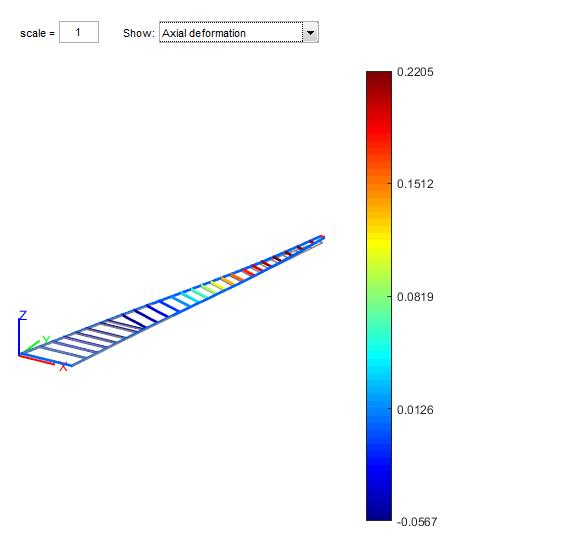
\includegraphics[width=0.6\textwidth]{img/AxialDeformation.jpg}
	\caption{Axial deformation (m)}
	\label{fig:axial_disp}
\end{figure}

\begin{figure}[h]
	\centering
	\begin{subfigure}{0.45\textwidth}
		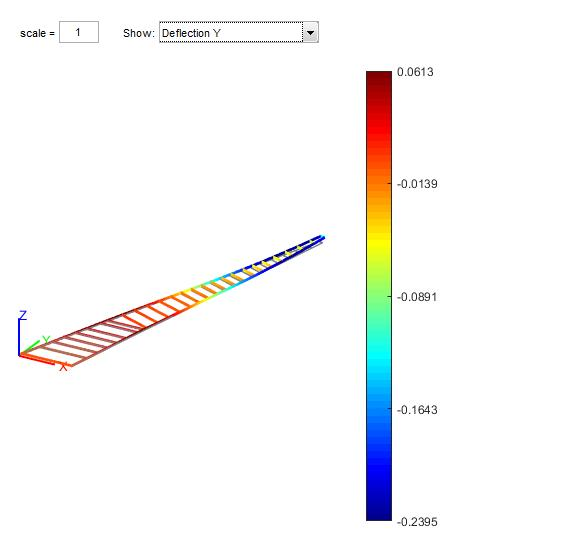
\includegraphics[width=\textwidth]{img/DeflectionY.jpg}
		\caption{Y axis}
		\label{fig:defl_y}
	\end{subfigure}
	~ %add desired spacing between images, e. g. ~, \quad, \qquad, \hfill etc.
	%(or a blank line to force the subfigure onto a new line)
	\begin{subfigure}{0.45\textwidth}
		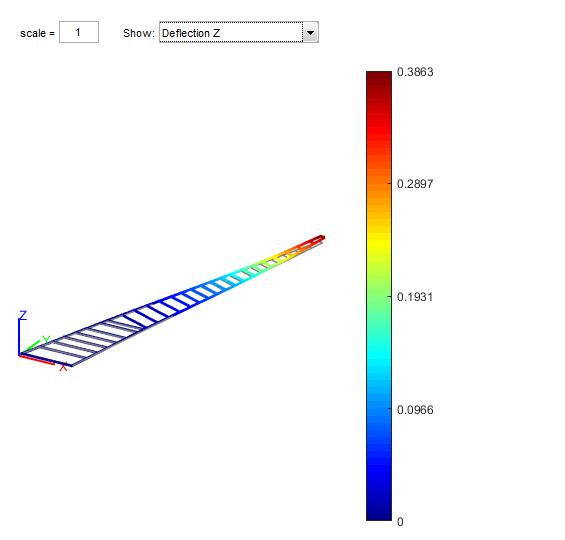
\includegraphics[width=\textwidth]{img/DeflectionZ.jpg}
		\caption{Z axis}
		\label{fig:defl_z}
	\end{subfigure}
	\caption{Deflections in local axis}
	\label{fig:deflections}
\end{figure}

\begin{figure}[h]
	\centering
	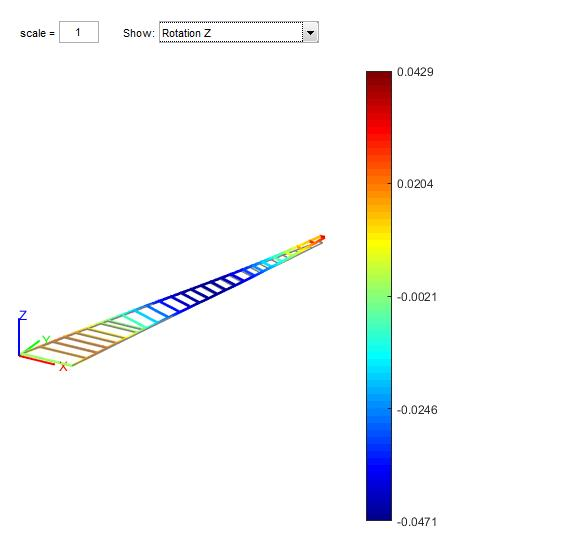
\includegraphics[width=0.6\textwidth]{img/RotationZ.jpg}
	\caption{Rotation in Z axis}
	\label{fig:rot_z}
\end{figure}

\begin{figure}[h]
	\centering
	\begin{subfigure}{0.45\textwidth}
		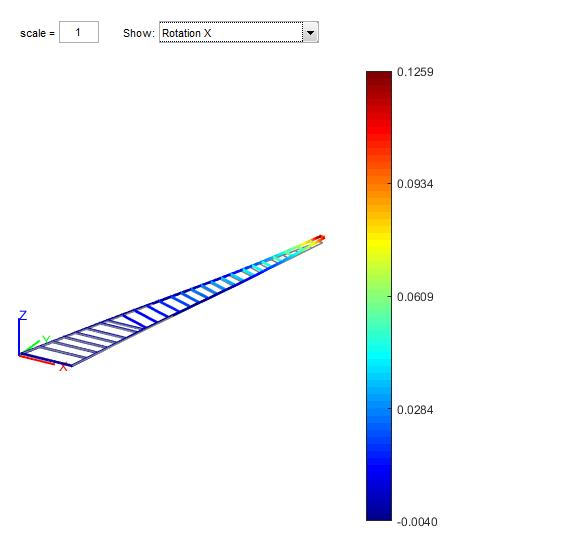
\includegraphics[width=\textwidth]{img/RotationX.jpg}
		\caption{X axis}
		\label{fig:rot_x}
	\end{subfigure}
	~ %add desired spacing between images, e. g. ~, \quad, \qquad, \hfill etc.
	%(or a blank line to force the subfigure onto a new line)
	\begin{subfigure}{0.45\textwidth}
		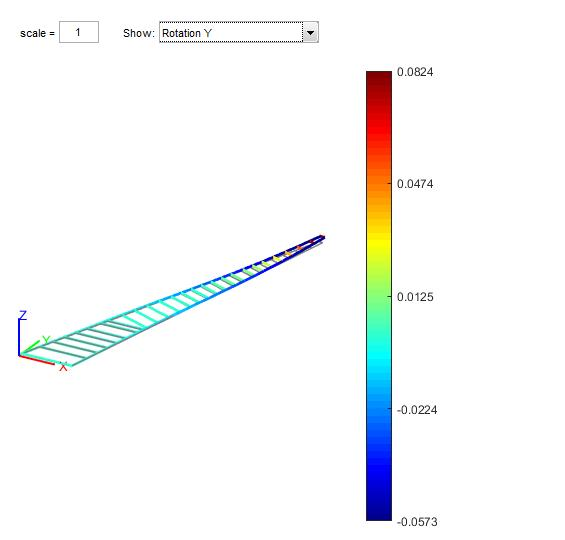
\includegraphics[width=\textwidth]{img/RotationY.jpg}
		\caption{Y axis}
		\label{fig:rot_y}
	\end{subfigure}
	\caption{Section rotations angles}
	\label{fig:rotations}
\end{figure}

\begin{figure}[h]
	\centering
	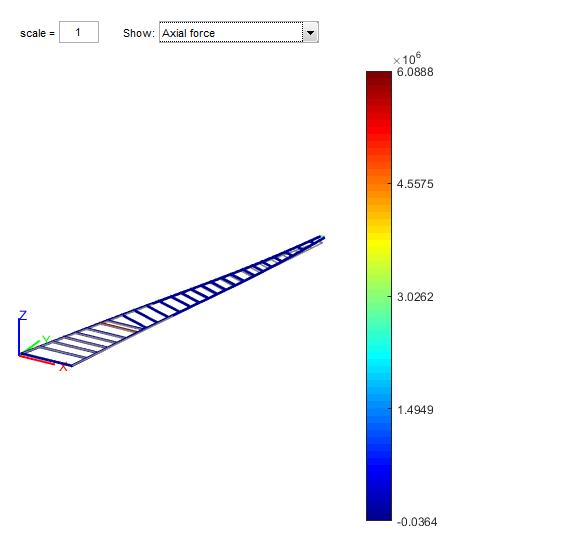
\includegraphics[width=0.6\textwidth]{img/AxialForce.jpg}
	\caption{Axial forces (N)}
	\label{fig:axial_force}
\end{figure}

\begin{figure}[h]
	\centering
	\begin{subfigure}{0.45\textwidth}
		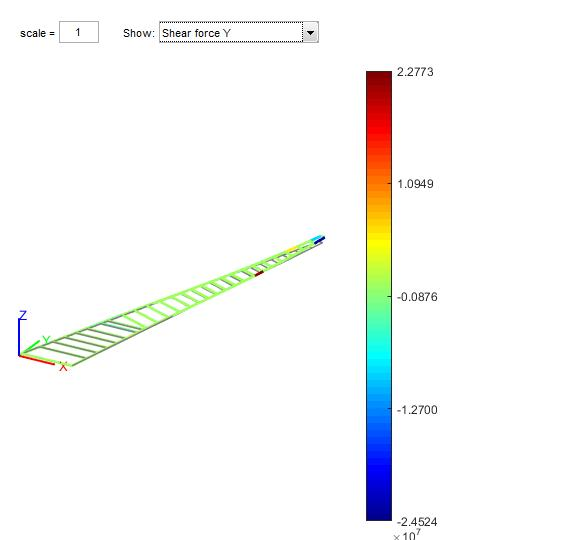
\includegraphics[width=\textwidth]{img/ShearForceY.jpg}
		\caption{Y axis}
		\label{fig:shear_y}
	\end{subfigure}
	~ %add desired spacing between images, e. g. ~, \quad, \qquad, \hfill etc.
	%(or a blank line to force the subfigure onto a new line)
	\begin{subfigure}{0.45\textwidth}
		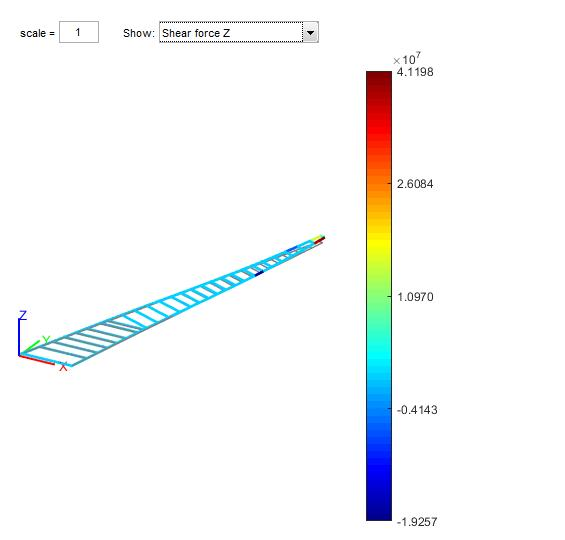
\includegraphics[width=\textwidth]{img/ShearForceZ.jpg}
		\caption{Z axis}
		\label{fig:shear_z}
	\end{subfigure}
	\caption{Shear forces}
	\label{fig:shear}
\end{figure}

\begin{figure}[h]
	\centering
	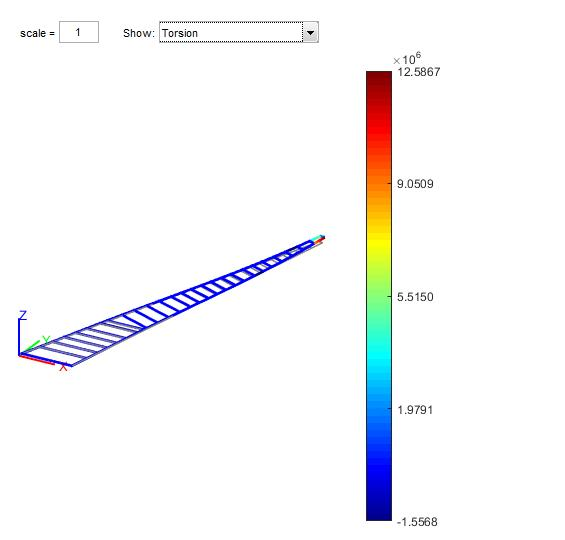
\includegraphics[width=0.6\textwidth]{img/Torsion.jpg}
	\caption{Torsional moment}
	\label{fig:torsion}
\end{figure}

\begin{figure}[h]
	\centering
	\begin{subfigure}{0.45\textwidth}
		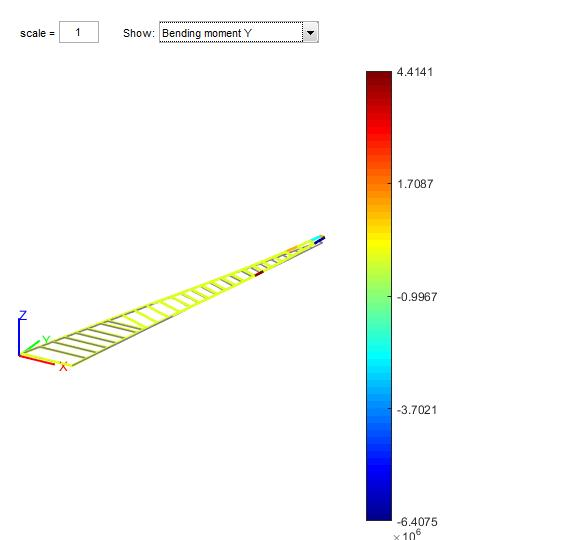
\includegraphics[width=\textwidth]{img/BendY.jpg}
		\caption{Y axis}
		\label{fig:bending_y}
	\end{subfigure}
	~ %add desired spacing between images, e. g. ~, \quad, \qquad, \hfill etc.
	%(or a blank line to force the subfigure onto a new line)
	\begin{subfigure}{0.45\textwidth}
		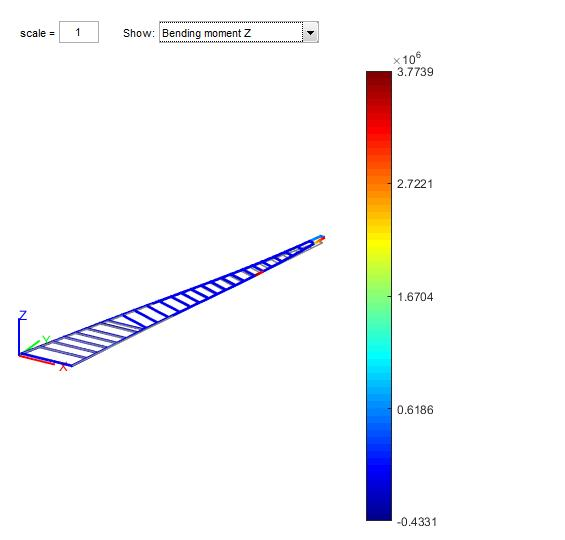
\includegraphics[width=\textwidth]{img/BendZ.jpg}
		\caption{Z axis}
		\label{fig:bending_z}
	\end{subfigure}
	\caption{Bending moments}
	\label{fig:bending}
\end{figure}

\clearpage

\section{Discussion of the results}

Observing figure \ref{fig:displacements} we can assume that the values are close
to the expected results because the displacements are relatively small compared
with the size of the wing, and the main displacement contribution is made
in the positive-z axis, showing the effect of the lift over the whole wing, but with
a cumulative major effect at the tip of the wing.\\

This is also confirmed by figure \ref{fig:defl_z}, which shows the major displacement
in Z direction at the tip of the wing, while in the middle, close to the engine position,
its weight compensates the lift and the displacement keeps close to zero.\\

Figure \ref{fig:rot_z} is also a good representation of the expected results.
It shows the rotation suffered by nodes in its Z-component. From the joints with the
fuselage to the pylon where the engine is attached, it can be seen a positive value,
meaning that it tries to rotate in anti-clockwise direction. This is mainly due to
the engine thrust, applied towards the forward direction. Then in the rest of the wing,
the main ration force is the drag, so the rotation is in the opposite sense, showing
negative values.\\

Figure \ref{fig:axial_force} shows that the force suffered by the ribs where the
engine is attached are much larger than in the rest of bars.\\
